\begin{savequote}[75mm]
The man who is swimming against the stream knows the strength of it.
\qauthor{Woodrow Wilson}
\end{savequote}

\chapter{Stream Processing}
Steams are older then computers so it is not a big surprice that streams
and the processing of them isn't a absolutly new topic in the computer science world.
Historically there are techniques like \textbf{logging} or in the domain driven development area there is \textbf{event sourcing},
which are very similar to streaming processing.
But they have not always been such an important deal like they is today with the with the unbelievable amount of data.
Antecedent to handle this streams was an event driven way and do analytics after storing the data.\\

\newpage

\section{Frozen yogurt}
Let me explain the \textit{old} event driven way with a small example.\\
Imagine a factory which produces frozen yogurt in different flavors.
They weigh and register every cup of yogurt at the end of the assembly line.\\

\begin{figure}[H]
\centering
\captionsetup{justification=centering}
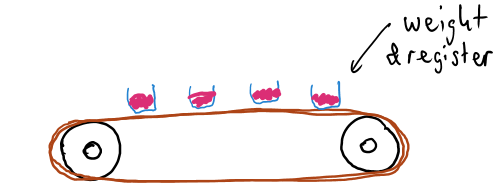
\includegraphics[width=0.5\textwidth]{images/cups.png}
\caption[Frozen yogurt assembly line]{frozen yogurt assembly line}
\end{figure}

\subsection{Common architecture}
The factory has sensors which weight the cups and this weights are sent to a server.
The server handles the request and stores the frozen yogurt with his weight in the database.
for analytic tasks there is a web application. If you are now interested in the total amount of produced cups.
You can simply open the browser go to the analytic page.
This starts a request to the server and the server will call the database with a quey like "select count(*) from frozen\_yogurt".
After the quey is executed you will get the result from the server and have the aggregated nummer on your screen.\\
(This is more or less a default example of a Three-tier architecture)

\begin{figure}[H]
\centering
\captionsetup{justification=centering}
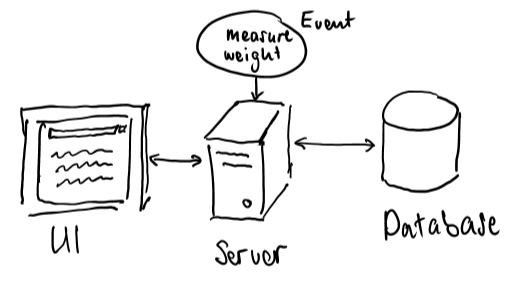
\includegraphics[width=0.6\textwidth]{images/three_tier.png}
\caption[Three-tier architecture]{Three-tier architecture}
\end{figure}

\newpage

Now the owner of the factory does a very good business and they are able to expand the production.
And with this expansion they also add a lot more of sensors to the assembly line like, a temperature sensor,
optical recognition to check if the cups are always full and a lot more.\\
The requirements of the system are also updated the owner want to have statistic about the production all the time
and want's immediately notifications if for example the temperature is to high.\\
These new requirements leads to new challenges in the architecutre of the system and are hard to implement with the
current state and the enormus data produced by the all sensors.

\begin{figure}[H]
\centering
\captionsetup{justification=centering}
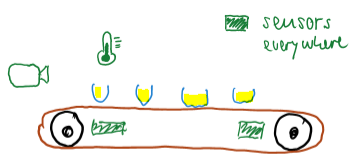
\includegraphics[width=0.6\textwidth]{images/sensors.png}
\caption[sensors everywhere]{sensors everywhere}
\end{figure}

\subsection{Streaming architecture}
A good way to handle this new requirements is to continuous aggregate and filter the stream of data before it is stored in the database.
For this purpose there has grown up a lot of new techniques and frameworks during the last few years.

\begin{figure}[H]
\centering
\captionsetup{justification=centering}
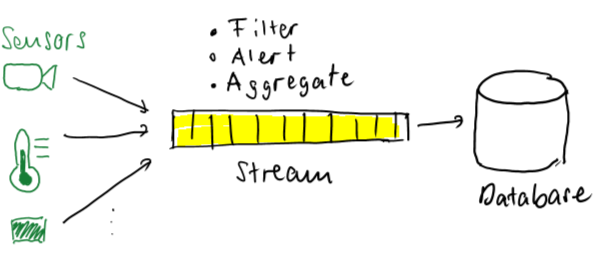
\includegraphics[width=0.6\textwidth]{images/stream.png}
\caption[streaming architecture]{streaming architecture}
\end{figure}
